\chapter{Definitionen}
\label{ch:chapter02}
Dieses Kapitel erklärt und beschreibt einige der zentralen Begriffe zum Thema des Hosts und der Berechtigungsstrukturen.
Dadurch soll der Leser ein Grundverständnis erhalten, um die folgenden Kapitel besser zu verstehen.

%
% Section: Der erste Abschnitt
%

\section{Host/Mainframe}
\label{sec:Host}
Der Host bzw. Mainframe ist ein Komplex aus verschiedenen Hochleistungscomputern.
Der Anbieter "`IBM"' definiert diesen dabei wie folgt: 
\newline
\newline
\textit{"`At their core, mainframes are high-performance computers with large amounts of memory and processors that process billions of simple calculations and transactions in real time."'} \cite{Mainframe}
\newline
\newline
Oder übersetzt:
\newline
\newline
\textit{"`Im Kern besteht der Mainframe aus Hochleistungsrechnern, welche über einen großen Speicher verfügen, und in der Lage sind Milliarden von einfachen Prozessen und Transaktion in Echtzeit durchzuführen."'} \cite{Mainframe}
\newline
\newline
Dabei spielt der Mainframe eine wichtige Rolle in der Finanzindustrie, welche widerstandsfähige, sichere und agile Server benötigt.
Dies ist der Fall, weil die Finanzindustrie über viele sensible Daten verfügt.
Daher müssen die Server sicher und widerstandsfähig sein, damit diese Daten nicht verloren gehen oder gestohlen werden.
Zudem müssen die Server agil sein, da die Technologie und die Regulierungen für den Mainframe sich stehtig ändern und dieser daher immer auf dem neuesten Stand sein muss.
Der Mainframe muss die Regularien vom \ac{VAIT} erfüllen, die von der \ac{BaFin} aufgestellt werden.
Die \ac{BaFin} soll eine konsistente IT-Strategie vorgeben, an die sich die Unternehmen halten müssen. \cite{Vait}

\section{Berechtigung}
\label{sec:Berechtigung}
Dabei definiert die \ac{NIST}, welche eine Institution von amerikanischer Regierung ist, Berechtigungen wie folgt:
\newline
\newline
\textit{"`The right or a permission that is granted to a system entity to access a system resource."'} \cite{Auth}
\newline
\newline
Dies bedeutet:
\newline
\newline
\textit{"`Das Recht oder die Erlaubnis haben, um auf System Ressourcen einer Systemeinheit zu zugreifen."'} \cite{Mainframe}
\newline
\newline
Im Kontext des Mainframebereiches betrifft dies bei Helvetia hauptsächlich das Betrachten und Zugreifen über Dialogmasken auf Daten.
\begin{figure}[h!]
 \centering
 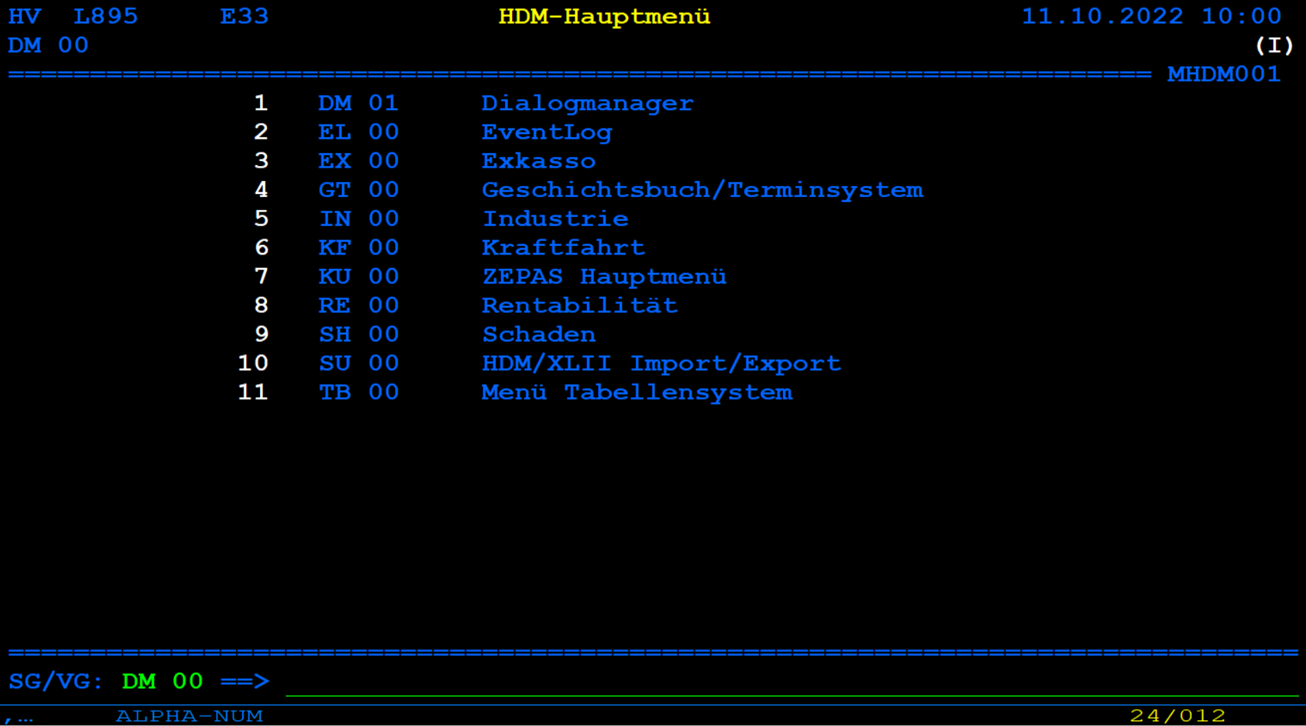
\includegraphics[width=1\textwidth]{gfx/Picture/Dialog.PNG}
 \caption{Beispiel Dialogmaske}
 \label{fig:Dial}
\end{figure}
Die Graphik (\ref{fig:Dial}) zeigt ein solches Dialogmaske.
Anhand dieser Dialogmaske kann man erkennen, dass der Nutzer L895 für die aufgezählten weiteren Dialogmasken (EL 00, EX 00, ...) zumindest die Leseberechtigung hat.
Zudem hat dieser die Schreibberechtigungen auf die Dialogmaske DM 00, da dieser sich in dieser Maske aufhält. 
\newline
\newline
\begin{figure}[h!]
 \centering
 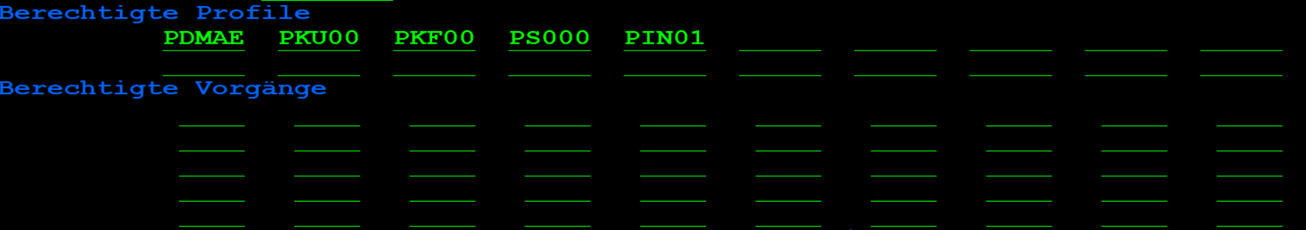
\includegraphics[width=1\textwidth]{gfx/Picture/Berechtigung.PNG}
 \caption{Berechtigungsdialogmaske}
 \label{fig:Berch}
\end{figure}
In dieser Graphik (\ref{fig:Berch}) kann man die Profile und individuellen Berechtigungen sehen, die der Nutzer L895 besitzt.
Dabei sind Profile Container für Berechtigungen.  \textbf{\textcolor[rgb]{1,0,0}{Dieser Satz muss umgeschrieben werden.}}

\section{Berechtigungsstruktur}
\label{sec:Berechtigungsstruktur}
Eine Berechtigungsstruktur besteht aus den Berechtigungen, die im Unterkapitel (\ref{sec:Berechtigung}) definiert werden, und aus der Struktur.
Dabei definiert Oxford Struktur wie folgt:
\newline
\newline
\textit{"`the way in which the parts of something are connected together, arranged or organized; a particular arrangement of parts"'} \cite{Struct}
\newline
\newline
Dies bedeutet, dass die Teile miteinander verknüpft, angeordnet oder organisiert sind. \cite{Struct}
\newline
In diesem Zusammenhang bedeutet Berechtigungsstruktur die Verknüpfung, Anordnung oder Organisation von Berechtigungen.
\begin{figure}[h!]
 \centering
 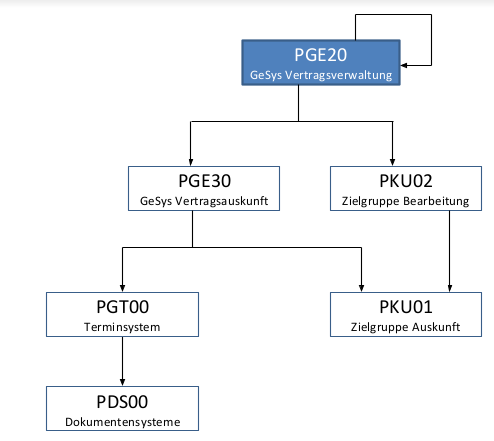
\includegraphics[width=1\textwidth]{gfx/Picture/Struktur.PNG}
 \caption{Teilausschnitt der Berechtigungsstruktur der Helvetia}
 \label{fig:Teil}
\end{figure}
Wie man in der Graphik (\ref{fig:Teil}) erkennen kann, sind die Profile hierarchisch aufgebaut.
Diese Profile beinhalten die Berechtigungen.
Daher ist die aktuelle Berechtigungsstruktur hierarchisch bei der Helvetia.


\section{IAM}
\label{subsec:IAM}
Die Virginia IT Agency beschreibt IAM wie folgt: Das \ac{IAM} ist eine Möglichkeit, sämtliche Nutzer und Profile, welche man zu den jeweiligen Personen über die IT-Umgebung über Nutzerrollen und Businessregeln zu ordnen kann, zu handhaben. Dabei ist die Zugriffverwaltung die Möglichkeit die Zugriffskontrolle über Regeln auf verschiedenen Plattformen einzuhalten. Ein wichtiger Teil von \ac{IAM} ist sicherzustellen, dass die Nutzer einen sicheren Zugriff auf die Ressourcen haben und auch nur auf die Ressourcen, die sie benötigen, um ihre Arbeit zu erledigen. \cite{Virg07}
\begin{figure}[h!]
 \centering
 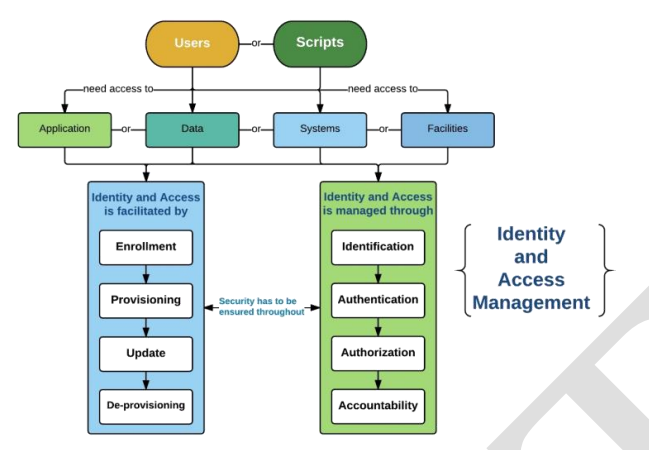
\includegraphics[width=1\textwidth]{gfx/Picture/IAM.PNG}
 \caption{Übersicht von IAM \cite{Moha19}}
 \label{fig:IAM}
\end{figure}
Im Bild (\ref{fig:IAM}) kann man erkennen, dass wenn ein Nutzer oder Programmzugriff auf eine Ressource möchte, dieser die Identifizierung, Authentifizierung, Autorisierung, sowie Rechtschaffenheit vorlegen und einhalten muss. \cite{Moha19}
\newline
Im Rahmen dieser Ausarbeitung handelt es sich bei den Ressourcen, um die Berechtigungen (\ref{sec:Berechtigung}).
